\section{SfM}
	\definition{SfM问题} 也称为\textbf{欧式结构恢复问题},已知$m$张图片和对应的相机内参矩阵$K_i(i=1,\cdots,m)$,求解:
	\begin{itemize}
		\item \textbf{Structure}:$n$个三维点$X_j(j=1,\cdots\,n)$的坐标
		\item \textbf{Motion}:$m$个相机的外参数$R_i,T_i(i=1,\cdots,m)$
	\end{itemize}		
	
	如果没有额外信息,无法恢复出场景的绝对坐标(经纬度)、朝向及尺度,恢复的最好结果是与真实场景之间差一个相似变换;\\

	比如,如果知道场景中某两点之间的真实距离,则可恢复出场景的尺度,但依然无法确定绝对坐标和朝向。

	\subsection{平行视图}
		在传统两视图(\ref{two_stereo})重建场景,两个相机只有平移而无旋转,此时$R = \mathbf{I}$,基础矩阵可简化为,
		$$
			\mathbf{F} = [e^\prime]_{\times}K^{\prime}K^{-1}
		$$

		一般两个相机会采用相同的参数,此时$K = K^\prime$,基础矩阵可进一步简化为,
		$$
			\mathbf{F} = [e^\prime]_{\times}
		$$

		平行视图的场景,极点为无穷远点,极线都平行于基线,此时$e^\prime = (1,0,0)^T$,

		$$
			\mathbf{F} =  \begin{bmatrix}
				0\quad & 0\quad& 0\\
				0\quad & 0\quad& -1\\
				0\quad & 1\quad& 0
			\end{bmatrix}
		$$

		根据(\ref{f_inverse_e}),
		\begin{equation}
			p^\prime_d = dp + e^\prime = d(u+1/d,v,1)^T \label{disparity_pair}
		\end{equation}
		$$
			p^\prime_d = dp + e^\prime = d(u+1/d,v,1)^T
		$$

		此时,$p^\prime_u = u + 1/d, p^\prime_v = v$,即对应点的$v^\prime$坐标与原$v$坐标坐标是相同的,两条极线具有相同的高度,此时极线也称为\textbf{扫描线}。

		\begin{figure}[H]
			% \begin{center}
			\begin{minipage}[t]{0.49\linewidth}
				\centering
				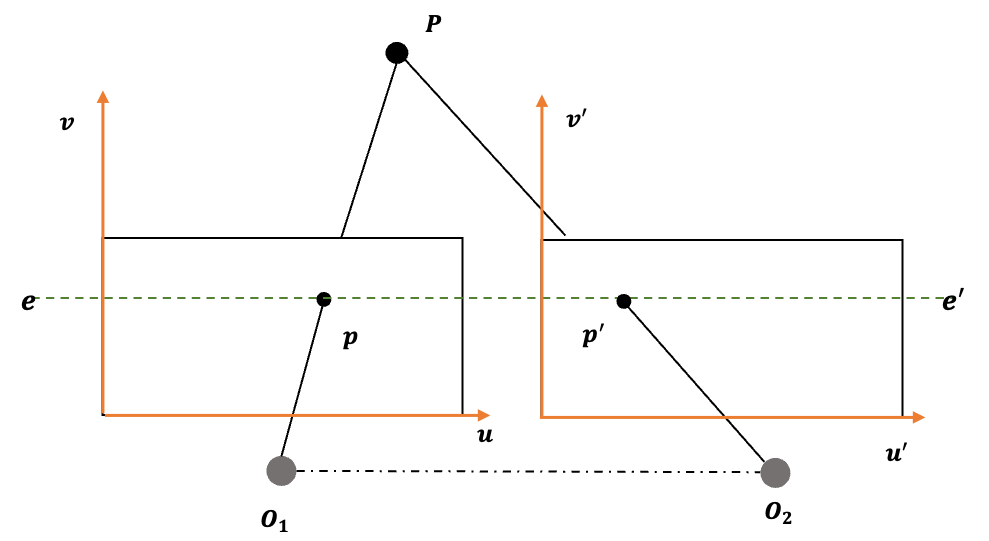
\includegraphics[width=\textwidth]{images/two_stereo.png}
				\caption{平行视图}
				\label{two_stereo}
			\end{minipage}
			\begin{minipage}[t]{0.49\linewidth}
				\centering
				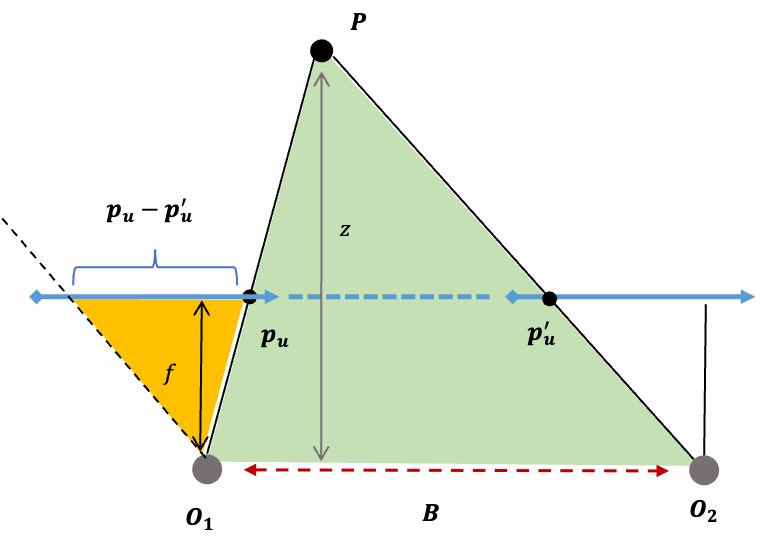
\includegraphics[width=\textwidth]{images/two_stereo_depth.png}
				\caption{平行视图俯视几何}
				\label{two_stereo_gemotry}
			\end{minipage}			
		\end{figure}

		沿着扫描线,平行视图的深度计算非常容易,如图(\ref{two_stereo_gemotry})两个三角形相似,可得,
		$$
			p_u - p^\prime_u = \frac{Bf}{z}
		$$

		$p_u - p^\prime_u$称为\textbf{视差},是同一3D点在两个成像平面的水平像素差。$B,f$均为已知量,以此知视差与深度成反比。

		\subsubsection*{极线校正}
			上面说的平行视图是非常理想的情况,实际上之前提到过,因为工艺的原因,很难保证单相机的像平面是矩形,也很难保证两个相机的像平面是绝对平移的;\\

			对此需要将两个像平面修正为平行平面,此时极线才能真正构成\textbf{扫描线},这个过程称为\textbf{极线校正}。具体来说,先把第二个平面的极点$e^\prime$变换到$(1,0,0)^T$,得到变换矩阵$H^\prime$;再利用投影误差最小化,得到第一个平面的变换矩阵$H$,如此可使得两极线对齐。具体细节请参考鲁鹏老师课程。
			\begin{figure}[H]
				\begin{center}
					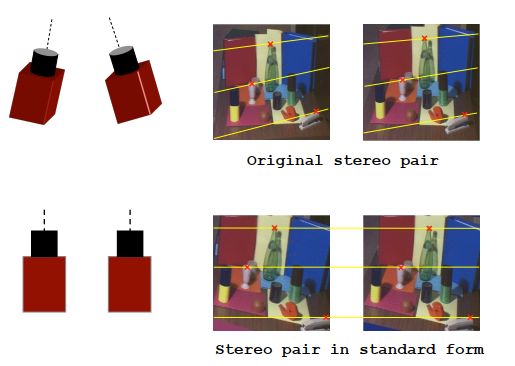
\includegraphics[width=0.8\textwidth]{images/epipolar.png}
				\end{center}
				\caption{极线校正}
			\end{figure}

		\subsubsection*{Matching Cost}
			根据(\ref{disparity_pair}),

			$$
				p_u - p^\prime_u = \frac{1}{d}
			$$

			视差与反投影距离$d$成反比,针对某个具体的点$p$,此处的$d$是某个确定的值$d_0$;\\

			不同的$d$会产生不同的视差,给$d$一个范围,逐一计算视差范围内的代价,每一代价$c_i$对应$p_i^\prime$。\\

			$w\times h$的图片,会产生$w\times h\times d$的的张量,称为\textbf{匹配代价},MVSNet的的\textbf{Cost Volume}实际是将这一概念从两视图推广到了多视图。\\

			\begin{figure}[H]
				\begin{center}
					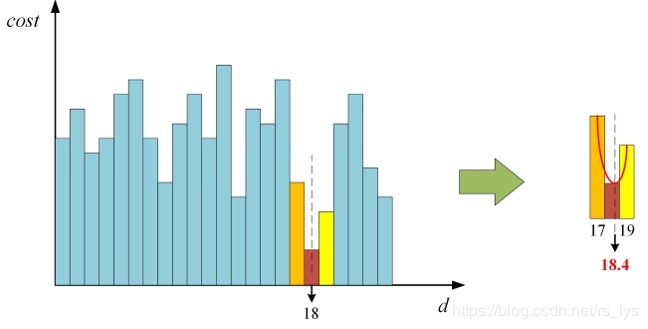
\includegraphics[width=0.85\textwidth]{images/matching_cost.jpeg}
				\end{center}
				\caption{Matching Cost \& 二次曲线修正\protect\footnote{\url{https://blog.csdn.net/rs_lys/article/details/83302323}}}
			\end{figure}

			那些平行于像平面的场景点深度是相同的,产生的视差也是相同的,这样的平面称也为\textbf{fronto-parallel}平面;\\

			而场景中的斜面(\textbf{slanted plane}),虽然也是平面,但上面点的深度是不同的,所以产生的视差也是不同的。\\

			在计算匹配代价时,像素视差误差会平方放大深度误差($d$为视差,$D$为深度),

			$$
				\Delta d= -\frac{Bf}{D^2}\Delta D \Rightarrow \Delta D = -\frac{D^2}{Bf}\Delta d
			$$
			
			所以需要通过视差变化来刻画点对之间的匹配程度,比如,视差变化很小的区域可能处在同一\textbf{fronto-parallel}平面;视差变化连续的区域可能处在同一\textbf{slanted plane}上;而视差变化剧烈的区域可能处在不同的曲面或曲率很大的曲面上。\\

			这是各种文献里都要对fronto-parallel plane、slanted plane及其他情况进行区分的原因。

		\subsubsection*{双目立体匹配}
			双目立体成本较低,一般用在自动驾驶或机器人场景,传统的匹配过程包括四个步骤:

			\begin{enumerate}
				\item 代价计算,具体就是衡量在两张图像上点对的匹配代价,代价可以是两点灰度绝对值差、绝对值和、归一化相关系数、互信息、Census变换、Rank变换等方法衡量;对匹配范围而已,主要是局部计算,可以点点计算,也可邻域匹配计算
				\item 代价聚合,通过局部或者全局的方式进一步调优上一步的匹配代价
					\begin{itemize}
						\item 局部方法,通过\textbf{支撑窗口}做均值滤波,又分为固定窗和自适应窗
						\item 全局方法,定义一个能量函数,最小化整体点点代价匹配,转化为一个优化问题
					\end{itemize}
				\item 视差计算,取代价最小的视差作为真值
				\item 视差优化,手段包括提高精度,比如上图通过二次曲线拟合将视差整数值扩展到浮点值;剔除错误匹配、弱纹理优化、填补空洞等
			\end{enumerate}

			最为提及的概念便是局部方法中的\textbf{support window},实际就是一个常见的邻域均值,以此抑制单点噪音。\\

			但窗内的像素可能因深度不同而导致视差不同,固定窗的均值滤波可能会因此引入视差噪音,从而放大深度误差,因此有一些自适应窗的方法来应对这个问题,这里不再展开。\\

			实际上,全局方法和局部方法一样,也暗含了邻域视差不变的假设\footnote{\url{http://vision.deis.unibo.it/~smatt/Seminars/StereoVision.pdf}}。


	\subsection{两视图重建}

	考虑两张图片,只要能估计出基础矩阵$F$,便可根据\ref{section_recovery_outer_p}节估计出$R,T$,
	$$
		p^\prime F p = 0
	$$

	根据基础矩阵约束,$p=(u,v,1)^T,p^{\prime} = (u^{\prime}, v^{\prime},1)$
	$$
		(u^{\prime}, v^{\prime},1)
		\begin{bmatrix}
			F_{11}\quad& F_{12}\quad& F_{13}\\
			F_{21}\quad& F_{22}\quad& F_{23}\\
			F_{31}\quad& F_{32}\quad& F_{33}\\
		\end{bmatrix}
		(u,v,1)^T = 0
	$$
	展开可得,

	$$
		\left(uu^{\prime}, vu^{\prime}, u^{\prime}, uv^{\prime},vv^{\prime},v^{\prime},u,v,1\right)
		\begin{bmatrix*}
			F_{11}\\
			F_{12}\\
			F_{13}\\
			F_{21}\\
			F_{22}\\
			F_{23}\\
			F_{31}\\
			F_{31}\\
			F_{33}
		\end{bmatrix*} = 0
	$$

	在不考虑尺度的情况下,$F$矩阵有8个未知数,因此至少需要8对点才能确定$F$,实际上会用大于8对点,求一个最小二乘解。\\

	$F$的秩为2,最小二乘解得到的矩阵秩一般为3,需要做一次SVD分解,置最小特征值为0,来得到$F$。

	\subsubsection*{解的存在性}
		并不是任意8对点都能求解出$F$,如果8个方程中部分线性相关,会导致方程的数量少于未知数的数量,从而没有唯一解。\\

		如果场景是一张平面,$P_i(i=1,2,3)$是平面上不共线的三点,对应像素坐标$p_i,p^\prime_i$;

		平面上任意点$P$可表示为$P_i$的线性组合,$P=\alpha P_1 + \beta P_2 + \gamma P_3$,$P$的投影为,
		
		\begin{align*}
			p &= K\left(\alpha P_1 + \beta P_2 + \gamma P_3\right)\\
				&= \alpha KP_1 + \beta K P_2 + \gamma KP_3\\
				&= p_1 + p_2 + p_3
		\end{align*}

		场景平面存在单应变换,
		$$
			p^\prime = Hp = Hp_1 + Hp_2 + Hp_3 = p^\prime_1+p^\prime_2+p^\prime_3
		$$

		因此,点对$(p_1 + p_2 + p_3,p^\prime_1+p^\prime_2+p^\prime_3)$贡献了一个冗余方程,此时基础矩阵没有唯一解,实际上要使得线性无关的方程数量至少为8,方程才有唯一解。\\

		在单应变换的情况下,需求解单应矩阵,单应矩阵包含了基础矩阵所有的元素,以此来构造基础矩阵。\\

		为了避免陷入讨论解的存在性,在重建场景时,经常用基础矩阵和单应矩阵分别求解一次,哪个效果好用哪个。

	\subsubsection*{确定对应点对}
		怎么确定两张图像的对应点对$p,p^{\prime}$?可以用传统的SIFT特征匹配,也可以用深度学习的方法,这里就不再详细介绍。

	
	注意这里世界坐标系选择为第一个相机的坐标系,因此只有第二个相机的$R,T$需要求解,得到基础矩阵$R,T$后,根据投影关系,
	$$
		P_d = dK^{-1}p
	$$

	可计算出空间点$P$的3D坐标,也称点云,这就是\textbf{三角化}方法。\\

	这个坐标是在第一个相机坐标系下的坐标,并且重建出的目标会跟真实大小相差一个尺度$d$。

	\subsection{多视图重建}
		多张图片,多个相机内参矩阵,求解SfM问题常用\textbf{增量法},具体来说包括几个步骤,
	
	\begin{itemize}
		\item 相机之间通过两视图方法两两求解$F_{ij}$
		\item 从一对相机开始,不断加入其他相机,这样重建的点会越来越多
		\item 持续加入相机会累积误差,所以通过\textbf{捆绑调整}(Bundle Adjustment)来做一个整体优化
	\end{itemize}

	其中细节和技巧非常多,具体请参考鲁鹏老师的课程\footnote{\url{https://www.bilibili.com/video/BV1Ss4y197CU}}(多视图重建一节)。\\

	这里要说的是这个\textbf{捆绑调整}方法,本质通过$L_2$距离最小化投影误差,
	$$
		E(M,X) = \sum_{i=1}^m \sum_{j=1}^n D\left(x_{ij}, M_iX_j\right)^2
	$$

	\begin{figure}[H]
		\begin{center}
			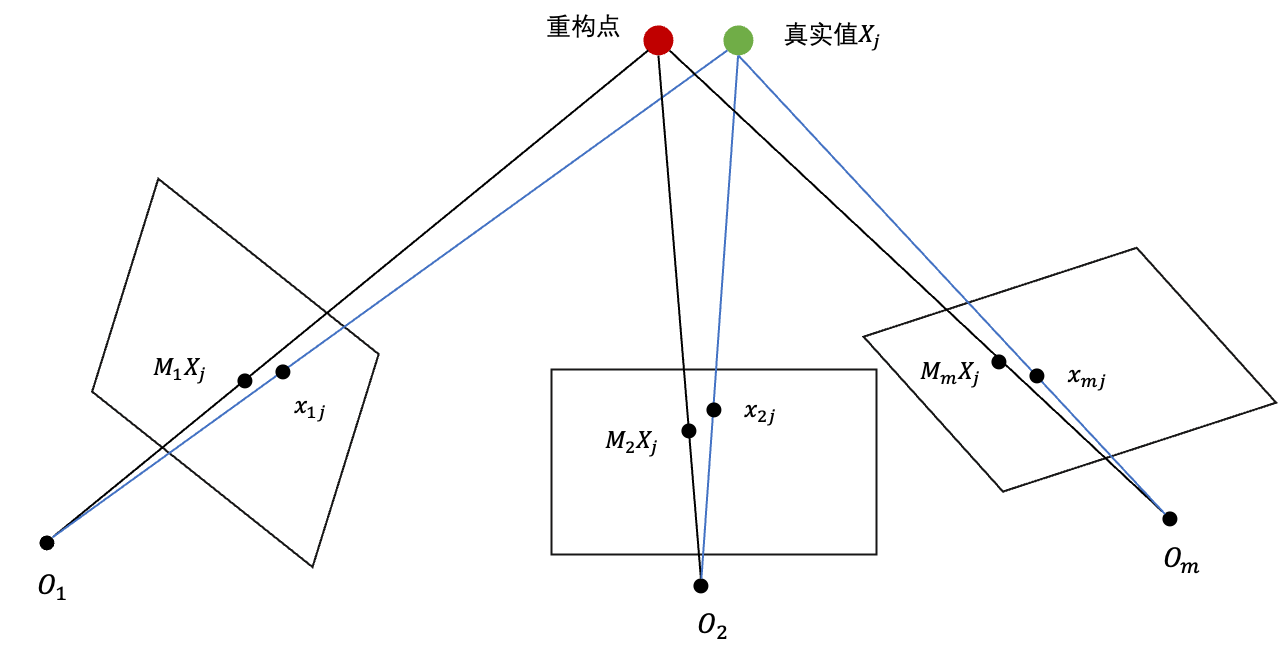
\includegraphics[width=\textwidth]{images/ba.png}
		\end{center}
		\caption{BA重投影误差}
	\end{figure}

	理论上可以通过梯度下降优化BA,直接得到$M,X$;实际上传统做法是先用增量法求的一个初解,再用BA方法优化,以加速收敛。\\

	如果样本足够多,将传统SfM转化为机器学习问题,效果也未必就差;但传统方法是对单场景重建,能收集的样本有限。\\

	图像上的点,至少被两个相机看到,构成点对的点才能计算出深度信息,如果两个相机姿态差距太大,会因为遮挡等原因导致可匹配的点减少。\\

	BA优势就是不需要所有的点都被所有的相机看到,每个相机只关注自己能看到点即可。